\documentclass[11pt]{article}
\usepackage[brazilian]{babel}
\usepackage[utf8]{inputenc} %acentuação da língua portuguesa
\usepackage[T1]{fontenc} 
\usepackage{wrapfig} %figura ao lado do texto
\usepackage{graphicx} %pacote de figuras

\usepackage{amsfonts} %pacote com \mathbb{}

\usepackage[pdftex]{hyperref} %links da internet

\usepackage{fancyhdr} 

\usepackage{hyphenat} %retirar hefenação

\tolerance=1 %retirar hefenação

\emergencystretch=\maxdimen %retirar hefenação

\hyphenpenalty=10000 %retirar hefenação

\hbadness=10000 %retirar hefenação

\hyphenchar\font=-1 %retirar hefenação

\sloppy %retirar hefenação

\usepackage{textcomp}

\usepackage[a4paper,left=2cm,right=2cm,top=2.5cm,bottom=2cm]{geometry}

\setlength{\parindent}{0pt} %Parágrafo sem identação]

\begin{document}
	
	\pagestyle{fancy}
	\renewcommand{\headrulewidth}{0pt}
	\renewcommand{\footrulewidth}{2.1pt}
	\fancyfoot[L]{\small Diego Silveira Costa Nascimento}
	\fancyfoot[R]{\small diego.nascimento@ifrn.edu.br}
	
	\begin{minipage}[c][1.5cm][c]{3cm}
		\begin{flushleft}
			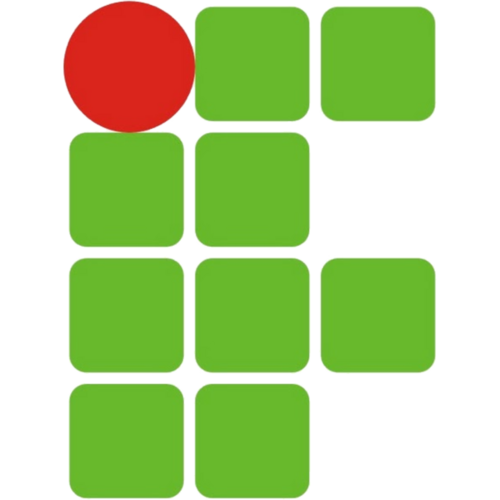
\includegraphics[scale=0.25]{IFRN}
		\end{flushleft}
	\end{minipage}		
	\begin{minipage}[c][1.5cm][c]{10.8cm}
		\begin{center}
			\resizebox{!}{0.3cm}{\textbf{Banco de Dados}}\par
			\resizebox{!}{0.2cm}{\textbf{Instituto Federal de Educação, Ciência e Tecnologia do Rio Grande do Norte}}\par
			\resizebox{!}{0.2cm}{\today}
		\end{center}
	\end{minipage}
	
	\begin{center}
		Exercícios
	\end{center}
	
	\section{Abordagem Entidade-relacionamento}
	
	\begin{enumerate}
		
		\item O que é uma entidade?
		
		\item O que é um relacionamento?
		
		\item O que é cardinalidade de um relacionamento? Exemplifique cada tipo.
		
		\item O que é um atributo?
		
		\item O que é uma generalização? Exemplifique.
		
		\item O que é uma entidade associativa?
		
		\item Construa um diagrama de entidade-relacionamento para uma agenda de contatos.
		
		\item Construa um diagrama de entidade-relacionamento para o controle acadêmico de uma
		instituição de ensino.
		
		\item Construa um diagrama de entidade-relacionamento para um sistema de controle de estoque.
		
		\item Construa um diagrama de entidade-relacionamento para um sistema de vendas de um
		restaurante. 
		
	\end{enumerate}
	
	\newpage
	
	\section{Abordagem Relacional}
	
	\begin{enumerate}
		\item Abaixo aparece um esquema parcial para um banco de dados relacional. Identifique neste
		esquema as chaves primárias e as chaves estrangeiras: 
		
		Aluno (codigo\_aluno, nome, codigo\_curso)\\
		Curso(codigo\_curso, nome)\\
		Disciplina(codigo\_disciplina, nome, creditos, codigo\_departamento)\\
		Curriculo(codigo\_curso, codigo\_disciplina, obrigatoria\_opcional)\\
		Conceito(codigo\_aluno, codigo\_disciplina, ano\_Semestre, conceito)\\
		Departamento(codigo\_departamento, nome)
		
		\item Levando em consideração o esquema de banco de dados apresentado na primeira questão, quais
		as restrições de domínios aplicadas em cada campo de todas as tabelas.
		
		\item Para o banco de dados cujo esquema está definido abaixo, explique que verificações devem ser
		feitas pelo SGBD para garantir integridade referencial nas seguintes situações: 
		
		a) Uma linha é incluída na tabela consulta.\\
		b) Uma linha é excluída da tabela paciente.\\
		
		paciente(codigo\_convenio, numero\_paciente, nome)\\
		codigo\_convenio referencia convenio\\
		convenio(codigo\_convenio, nome)\\
		medico(CRM, nome, especialização)\\
		consulta(codigo\_convenio, numero\_paciente, CRM, data\_hora)\\
		(codigo\_convenio, numero\_paciente) referencia paciente CRM referencia Medico 
	\end{enumerate}
	
	\newpage
	
	\section{Normalização}
	
	\begin{enumerate}
		\item Aplicar as regras de normalização cabíveis as tabelas:
		
		a) Empregado (Número Empregado, Nome do Empregado, Número do Departamento, Nome
		do Departamento, Número do Gerente, Nome do Gerente, Número do Projeto, Nome do
		Projeto, Dia de Início do Projeto, Número de horas trabalhadas no projeto).\\
		b) Ordem\_Compra (cd\_ordem\_compra, dt\_emissão, cd\_fornecedor, nm\_fornecedor,
		endereço\_fornecedor, cd\_material (n vezes), descrição\_material (n vezes), qt\_comprada (n
		vezes), vl\_unitário (n vezes), vl\_total\_item (n vezes), vl\_total\_ordem).\\
		c) Tabela de Notas Fiscais (Num\_NF, Série, Data emissão, Cod. Cliente, Nome cliente,
		Endereço cliente, CGC cliente, Código Mercadoria, Descrição Mercadoria, Quantidade
		vendida, Preço de venda, Total da venda da Mercadoria e Total Geral da Nota). Cada nota pode
		ter mais do que uma mercadoria.\\
		d) Inscrição (Código do Aluno, Nome do Aluno, Telefone para contato, Ano de Admissão,
		Código da Disciplina, Nome da Disciplina, Nome do Curso, Data da Matricula).\\
		e) Paciente (num\_paciente, nome\_paciente, num\_quarto, descrição\_quarto,
		num\_cômodos\_quarto, cod\_médico, nome\_médico, fone\_médico).\\
		f) Notas (matrícula\_aluno, nome\_aluno, endereço\_aluno, cod\_disciplina, desc\_disciplina,
		num\_crédito,nota, ano, período).
		
		\item Considere a Relação R (A,B,C,D,E,F) onde a chave primária é A,B e que apresenta as seguintes
		dependências funcionais: A => C, B => D, (A,B) => E, E => F.
		
		a) Dizer em forma Normal R se encontra; e\\
		b) Normalizar R até a terceira forma normal justificando cada etapa. 
		
		\item Considere R( A, B, C, D, E ) uma relação com as seguintes características: Dependências
		Funcionais : (C, D) -> A, A -> B, A-> E . Chave candidata : ( C, D ) . Pede-se, justificando a
		resposta:
		
		a) Informar em que forma normal R se encontra; e\\
		b) Normalizar R até 3 FN.
		
		\item Considere o esquema relacional composto pelas seguintes tabelas:
		
		Vendedor ( codvendedor, nome, data\_contrato, local\_trabalho, supervisor, salário, comissões )\\
		Cliente ( codcliente, nome, endereço, cidade, cep )\\
		Armazenagem ( codpeça, local, descrição, custo\_unitário, estoque)\\
		Fatura ( codfatura, codpeça, quantidade, data\_venda, codvendedor, codcliente )\\
		
		Sabendo-se que são válidas, entre outras, as seguintes dependências funcionais:
		codvendedor -> salário, comissões\\
		codpeça, local -> estoque\\
		local\_trabalho -> supervisor\\
		codfatura -> data\_venda, codvendedor, codcliente\\
		codpeça -> descrição, custo\_unitário\\
		codfatura,codpeça -> quantidade 
		
		Quais correções, você faria nas tabelas acima de forma a levar o esquema para a 3FN?
		
		\item Considere a seguinte relação para livros publicados:
		
		Livro (titulo, autor, tipo, preço, editora, país\_origem)\\
		Suponha que existam as seguintes dependências funcionais:\\
		Titulo - editora, tipo\\
		Tipo - preço\\
		Autor - país\_origem\\
		
		Responda:\\
		a) Em que forma normal a relação livro se encontra?\\
		b) Normalize até a 3FN, caso seja necessário.  
	\end{enumerate}
	
	\newpage
	
	\section{Structured Query Language (SQL)}
	
	\begin{enumerate}
		\item Criar um banco de dados chamado agenda.
		
		\item Criar a tabela de contatos com os campos código, nome, telefone, endereço.
		
		\item Referente à segunda questão, inserir os resultados a seguir.
		1, João, 9999-9999, Natal\\
		2, Maria, 8888-9999, Fortaleza\\
		3, Pedro, 8989-8888, Fortaleza\\
		4, Lucas, 8686-9191, Rio de Janeiro\\
		5, Sandro, 3322-5555, Maceió\\
		6, Mário, 2233-3322, Recife\\
		7, Ana, 2323-2323, Bahia\\
		8, Paulo, , Aracaju\\
		9, Marcos, ,\\
		10, José, 3333-2211 ,\\
		
		\item Adicionar uma coluna chamada sexo para a tabela da segunda questão, e fazer a atualização de
		cada registro de acordo com o sexo de casa pessoa.
		
		\item Atualizar o telefone de Paulo para 5555-2323.
		
		\item Atualizar o telefone e o endereço de Marcos, para 1122-3344 e São Paulo, respectivamente.
		
		\item Atualizar o endereço de José para João Pessoa.
		
		\item Excluir os contatos que moram em fortaleza.
		
		\item Selecionar o número do telefone de Lucas.
		
		\item Selecionar o endereço e o número do telefone de João.
		
		\item Criar as tabelas a seguir e aplicar as restrições de domínio.
		
		\textbf{tb\_cliente}
		\begin{itemize}
			\item código inteiro, não nulo e auto-incremento.
			\item nome, cadeia de caracter de tamanho 50.
			\item endereço, cadeia de caracter de tamanho 50.
			\item cidade, cadeia de caracter de tamanho 50.
			\item estado, caracter de tamanho 2.
			\item sexo, caracter.
			\item data de nascimento, date.
			\item salário, real.
			\item cpf, cadeia de caracter de tamanho 14.
			\item e-mail, cadeia de caracter de tamanho 30.
		\end{itemize}
		
		\textbf{tb\_projeto}
		\begin{itemize}
			\item código, inteiro, não nulo e auto-incremento.
			\item descrição, cadeia de caracter, não nulo.
			\item data de início, data.
			\item data de término, data.
		\end{itemize}
		
		\textbf{tb\_cliente\_projeto}
		\begin{itemize}
			\item código do cliente, inteiro e não nulo.
			\item código do projeto, inteiro não nulo.
			\item carga horária, inteiro.
		\end{itemize}
		
		\item Aplicar as restrições de chave para as tabelas da Questão 1:
		
		tb\_cliente (código);
		
		tb\_projeto (código) e
		
		tb\_cliente\_projeto (código do cliente, código do projeto).
		
		\item Aplicar as restrições de referencial para as tabelas da Questão 1:
		
		tb\_cliente\_projeto (código do cliente) referência a tb\_cliente (código)
		
		tb\_cliente\_projeto (código do projeto) referência a tb\_projeto (código)
		
		\item Aplicar as restrições de checagem para as tabelas da Questão 1:
		
		tb\_cliente (sexo) – Permitir apenas armazenar, M para o sexo Masculino e F para Feminino.
		
		tb\_cliente (salário) – Não pode ser menor igual a zero.
		
		tb\_projeto (data de término) – Não pode ser menor ou igual a data de início).
		
		tb\_cliente\_projeto (carga horária) – Não pode ser menor que 20 horas.
		
		\item Aplicar as restrições de unicidade para as tabelas da Questão 1:
		
		tb\_cliente (cpf)
		
		tb\_cliente (e-mail)
		
		\item Cria procedimentos para inserir dados em cada tabela (tb\_cliente,tb\_projeto, tb\_cliente\_projeto).
		
		\item Cria procedimentos para excluir dados em cada tabela (tb\_cliente,tb\_projeto, tb\_cliente\_projeto).
		
		\item Cria procedimentos para alterar dados em cada tabela (tb\_cliente,tb\_projeto, tb\_cliente\_projeto).
		
		\item Criar uma visão que selecione o código, nome e e-mail de todos os clientes.
		
		\item Criar uma visão que selecione o nome e endereços de todos os clientes.
		
		\item Criar uma visão que selecione o nome e salário de todas os clientes do sexo masculino.
		
		\item Criar uma função que recebe como parâmetro a siglas do sexo e retorne a descrição completa.
		
		\item Criar uma função que recebe como parâmetro a siglas de um estado e retorne a descrição completa.
		
		\item Criar uma função que receba como parâmetro a data de nascimento, e informe qual a idade do cliente.
		
		\item Criar um gatilho para validar o cpf de um contato quando o mesmo for inserido ou atualizado.
		
		\item Criar um gatilho para fazer um backup em uma tabela auxiliar dos clientes excluídos.
		
		\item Criar um gatilho que envie um e-mail ao administrador de banco de dados toda vez que um novo registro for incluído.
	\end{enumerate}
	
	\newpage
	\section{Consultas SQL}
	
	\centering
	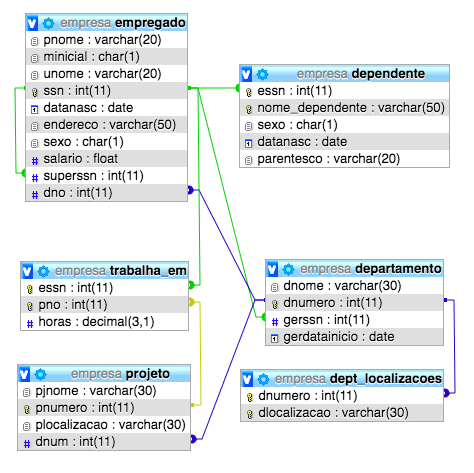
\includegraphics[scale=0.5]{empresa}
	
	\begin{enumerate}
		\item Selecione o nome completo de todos os empregados.
		
		\item Selecione o número e nome de todos os departamentos.
		
		\item Selecione o número, nome e a localização de todos os projetos.
				
		\item Selecione o ssn, nome e a data de nascimento (dd-mm-yyyy) dos empregados do sexo masculino.
		
		\item Selecione o nome de todos os empregados que não possuem supervisor.
		
		\item Selecione o nome de todos os dependentes que são cônjuge.
		
		\item Selecione todos os empregados que têm salário maior que 30000.
		
		\item Selecione todos os empregados do sexo femino e que ganham mais que 25000.
		
		\item Selecione todos os empregados que iniciem o nome pela letra J.

		\item Selecione todos os empregados que possui endereço em Houston.
				
		\item Selecione o nome e a data de nascimento (dd-mm-yyyy) de todos os dependentes que são cônjuge ou que são filho.
		
		\item Selecione o nome de todos os projetos que estão localizados em Stafford.
		
		\item Selecione o nome concatenado pelo último nome de todos os empregados do sexo feminino, que ganham mais de 3000 e que mora em Berry.
		
		\item Selecione todos os empregados que ganham salário entre 38000 e 43000.
		
		\item Selecione o número do departamento e a quantidade de empregados por sexo.
		
		\item Selecione o número do departamento e a quantidade de empregados por departamento.
		
		\item Selecione o número do departamento e a quantidade de projetos por departamento.
		
		\item Selecione o número do departamento e a média salarial por departamento.
		
		\item Selecione o sexo e os maiores salário por sexo.
		
		\item Selecione a soma de todos salários dos empregados que são do departamento 4.
		
		\item Selecione a média de todos os salários dos empregados que moram em Houston e que são do sexo masculino.
		
		\item Selecione o nome dos empregados e a quantidade de vezes que cada nome se repete.
		
		\item Selecione o tipo de parentesco dos dependentes e a quantidade de vezes em que cada tipo aparece.
		
		\item Selecione todos os empregados ordenados acesdentemente por nome.
		
		\item Selecione todos os empregados ordenados decrescentemente por idade.
		
		\item Selecione todos os empregados ordenado decrescentemento por salário, e ascendente por nome.

		\item Selecione todos os empregados que têm dependentes.		

		\item Selecione o nome e a data de nascimento dos empregados e o nome e a data de nascimento do
		do dependente cônjugue, em que a data de nascimento do empregado for menor que a data de
		nascimento do seu cônjugue.
		
		\item Selecione todos os empregados que trabalham em um projeto cujo departamento não é o seu.
		
		\item Selecione o ssn, o nome, e a diferença salarial em relação à média por sexo dos funcionários.
		
		\item Selecione o ssn e o nome todos os empregados que trabalham mais de 40 horas.
		
		\item Selecione o nome e a quantidades de dependentes de todos os funcionários.
		
		\item Selecione o ssn e o nome de todos os funcionários que trabalham apenas em projetos do próprio
		departamento.
		
		\item Selecione o ssn, nome e data de nascimento de todos os empregados que tem mais de um
		dependente, que trabalham mais de 5 horas e cujo departamento do projeto esteja em
		"Houston".
		
		\item Selecione o ssn, o nome dos empregados, o nome e total de horas trabalhadas por projeto.
		
		\item Selecione o ssn e o nome de todos os empregados que ganham mais que seu supervisor.
		
		\item Selecione o nome e salário dos empregados, e o nome e salário do supervisor, e a diferença de
		salários entre eles, para todos os empregados.
		
		\item Selecione o nome do projeto, o nome do departamento, sua localização e a quantidades de
		empregados que trabalham nele.
		
		\item Selecione o ssn e o nome de todos os empregados que gerenciam mais de um departamento.
		
		\item Selecione o ssn e nome dos empregados que gerenciam um departamento que não é o seu.
		
		\item Selecione o ssn e nome dos empregados que têm um casal de filhos.
	\end{enumerate}
	
\end{document}